\chapter{Modelling Evolution of Life-history Traits}

\section{Modelling Adult Stage}
After modelling larval stage and calibrating, I developed the model for the pupal and adult stage of \textit{Drosophila} life cycle. After larval stage, surviving individuals go through pupal stage where some of them undergo pupal mortality. The adult stage includes randomly choosing surviving adults from all replicate vials of pupal stage, matings, and inheritance of larval trait parameters from parents to offspring. Female is mated once with random male chosen from the adult population ($n$ = 2400) with replacement for simplicity. From all the offspring produced, eggs are chosen at random for the next generation with numbers respective to the crowding environment maintained.
\subsection{Pupal stage}
After collecting all the surviving individuals from the larval stage, a probability of death during pupal stage is assigned to each survived larva. This probability is dependent on the amount of waste accumulated in the body while econsuming food during the larval stage. This probability is given as:
\[P_{M}(i) = 1 - exp(-(W_{acum}(i) \cdot x_{3})^{2})\]
Here, \\
$P_{M}$ = Probability of dying during pupal stage \\
$W_{acum}(i)$ = Waste accumulated by $i^{th}$ larva during larval stage \\
$x_{3}$ = Scaling parameter
\subsection{Fecundity}
After each mating, the number of eggs produced for a female are derived from the fecundity equation based on the model of (ref) Tung S. (year). Fecundity is taken as a function of body size of the female and adult nutrition parameter (the amount of yeast provided). Fecundity of an $i^{th}$ female is given as:
\[Egg_{i} = Nut \cdot x_{3} \cdot \log{(x_{4} \cdot s_{i})}\]
Here, $s_{i}$ = body size of the $i^{th}$ female \\
$Egg_{i}$ = Number of eggs laid by the female in a mating \\
$Nut$ = Adult nutrition i.e. the amount of yeast provided \\
$x_{3}, x_{4}$ = scaling parameters
\subsection{Inheritance}
Larval trait parameters (initial feeding rate, effieciency, waste tolerance and critical size) are inherited from parents to offspring produced by each female using mid-parent value. The mid-parent value i.e. average of mother and father for each larval parameter of all offspring is calculated. This mid-parent value is taken as a mean of a normal distribution with fixed standard deviation for respetive trait parameters. The standard deviation in this normal distribution determines the heritibility of the mid-parent value and it is considered to be different for each trait parameter. Trait parameters of the offspring are assigned as:
\[T_{i} \in N(mpv_{T}, \delta_{T})\]
Here, \\
$T_{i}$ = Trait parameter assigned to $i^{th}$ offspring from a mating \\
$mpv_{T}$ = Mid-parent value of of the trait $T$ for a given mating \\
$\delta_{T}$ = heritability of mid-parent value of the trait $T$ \\
$N(mpv, \delta)$ = Normal distribution with $mpv$ as mean and $\delta$ as standard deviation
\begin{figure}[p]
  \centering
  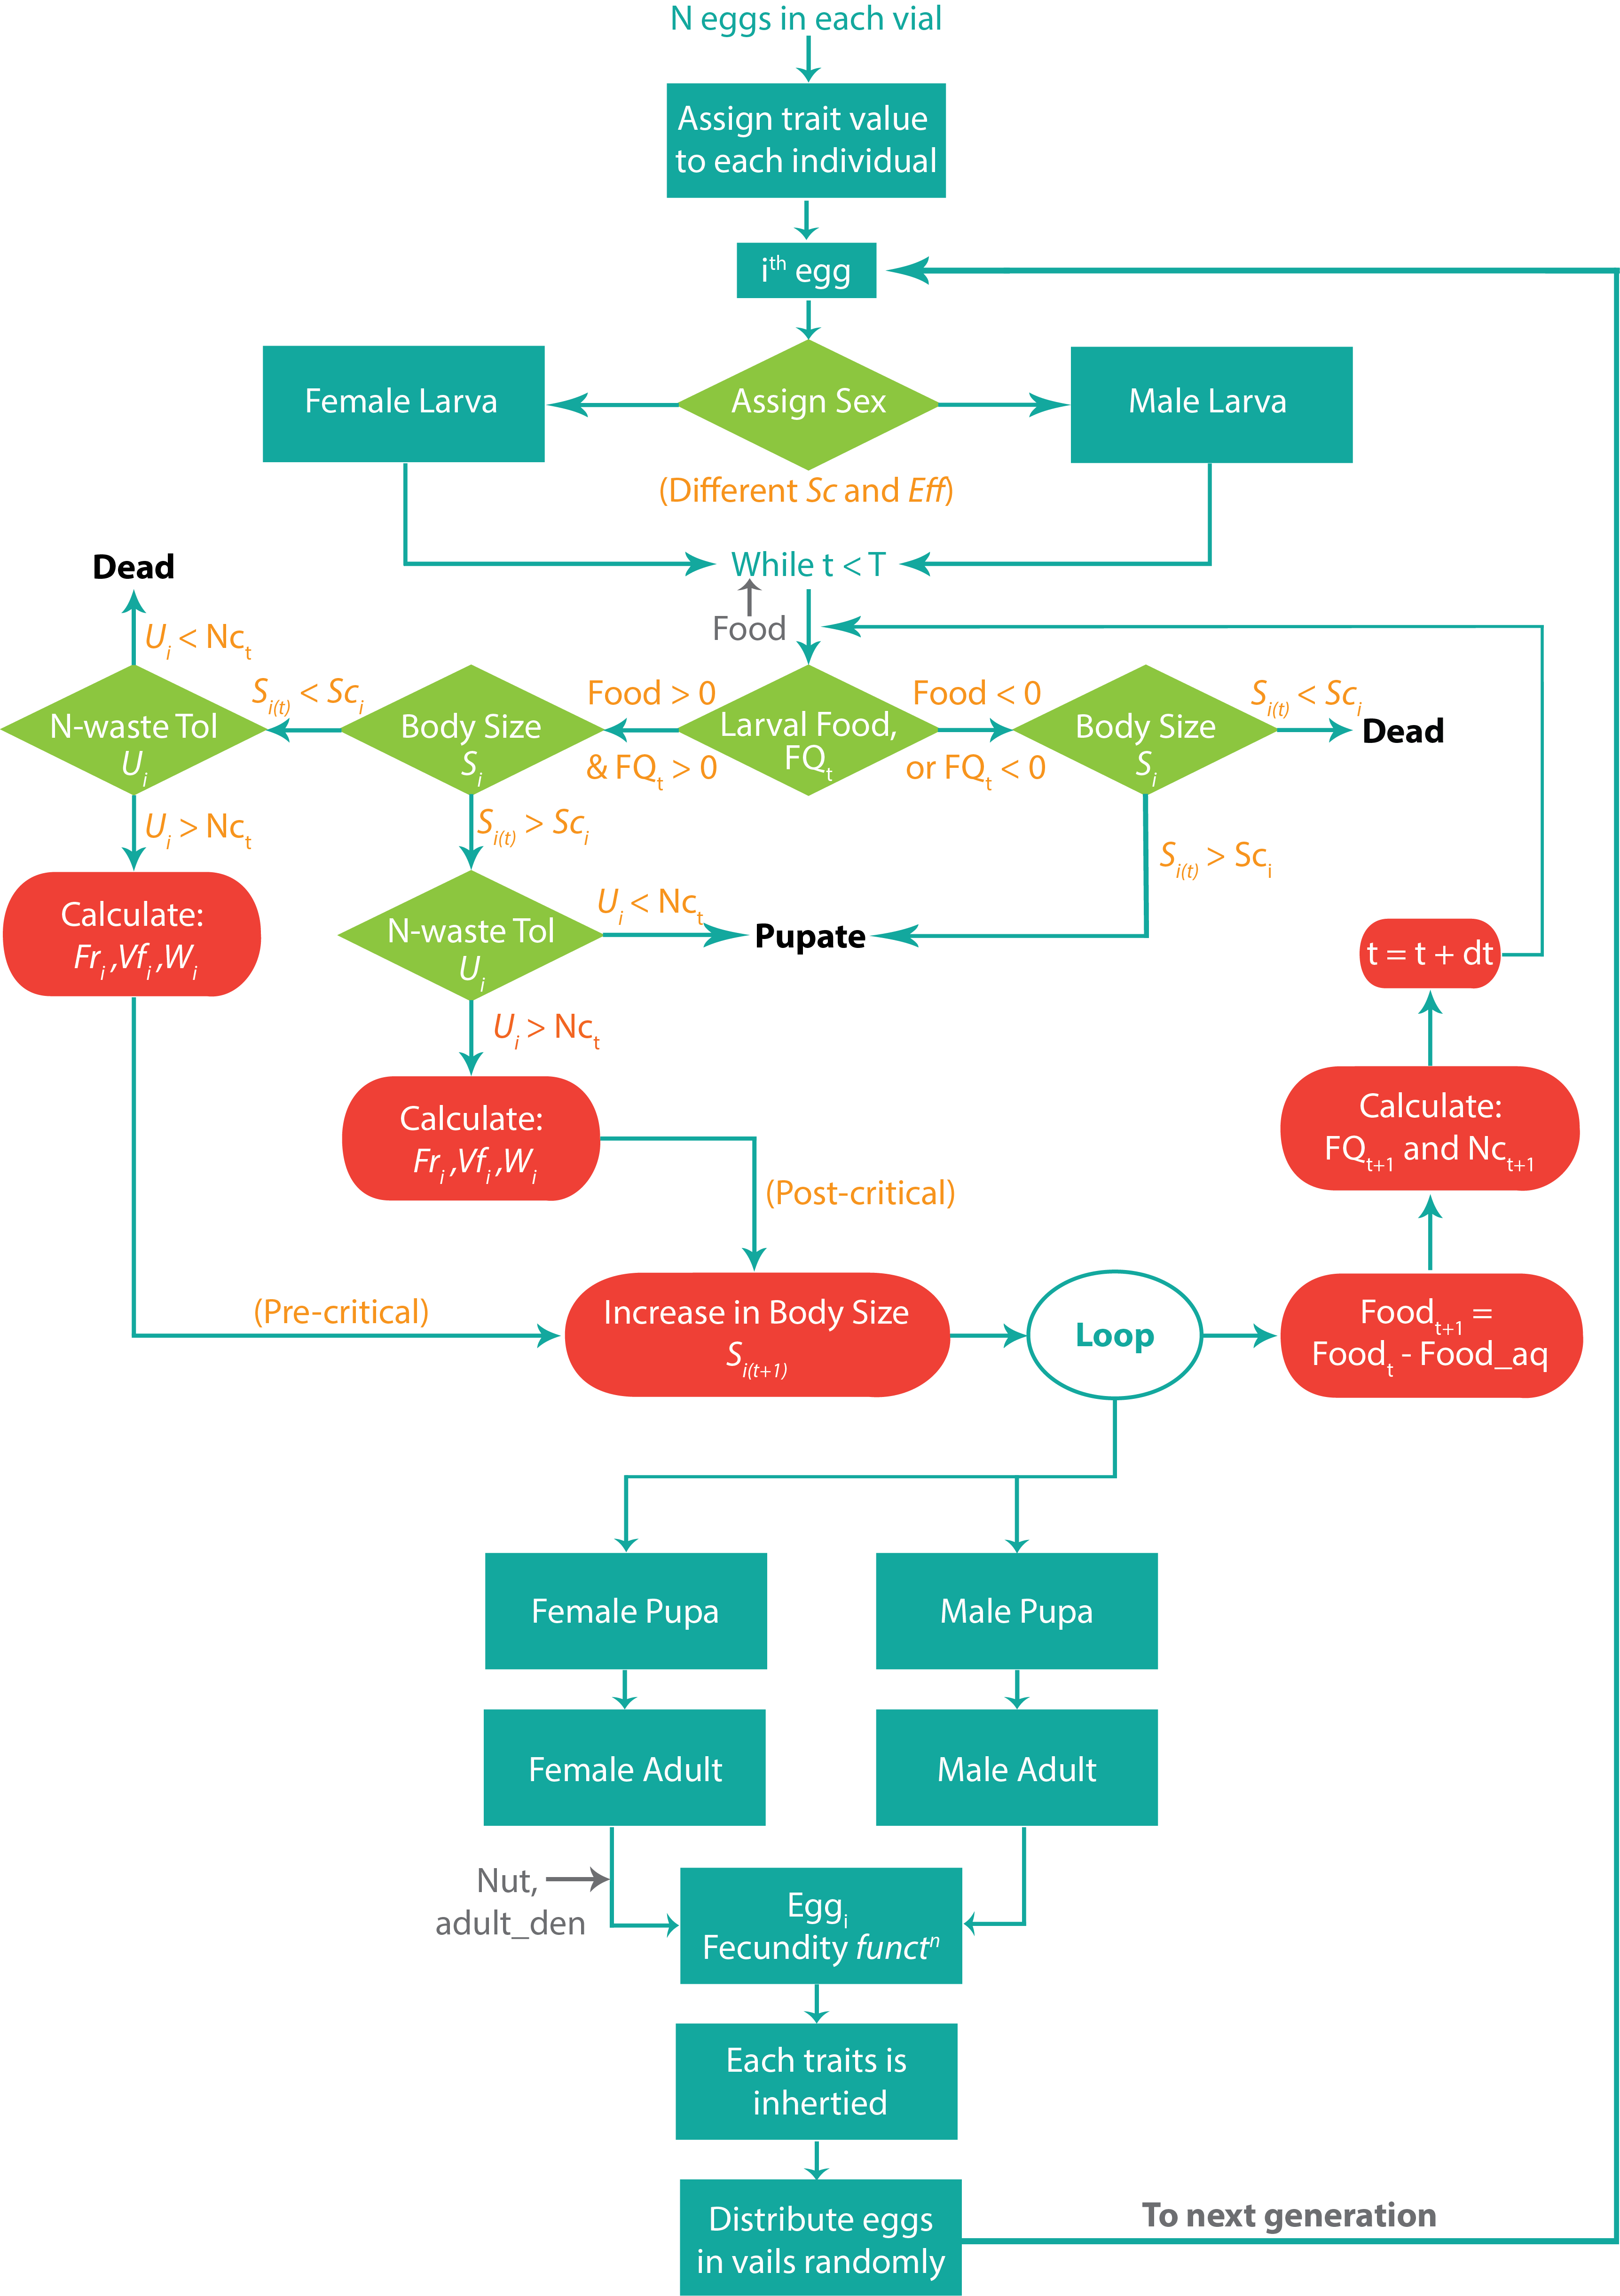
\includegraphics[trim= 0 0 0 0, clip, width= \textwidth]{C4/Figs/model}
  \caption{Model flowchart}
  \label{model}
\end{figure}

\newpage
\section{Effect of Laral Crowding on the Evolution of Life-history Traits}
Using values for all parameters given in table~\ref{tab:food_param} and table~\ref{tab:scale_param}, the entire model is simulated for 100 generations with 10 replicates for MB, MCU and CCU cultures. The overall model follows the path shown in fig~\ref{model}. All larval trait parameters are taken from independent distribution and there is no correlation between them (see table~\ref{tab:trait_value}). To see how larval trait parameters evolve over time, timeseries for these traits of surviving adult individuals are plotted with 95$\%$ CI.\\ \\
In MB culture, being control population, nonw of the parameters evolve over time (see fig~\ref{fr}, fig~\ref{eff}, fig~\ref{mc}, fig~\ref{wtol}). Initial feeding rate in high density cultures increase over generations at similar rate but inital feeding rate is higher always in CCU culture always than in MCU culture. Efficiency show similar trend in high density cultures i.e. it increases over generations at similar rate but is higher always in CCU culture always than in MCU culture. Critical size in high density cultures decreases at the same rate but critical size in CCU culture is always lower than in MCU culture. Waste tolerance does not evolve in all of the culture populations since there is no significant change in waste tolerance value.
\begin{figure}[h]
  \centering
  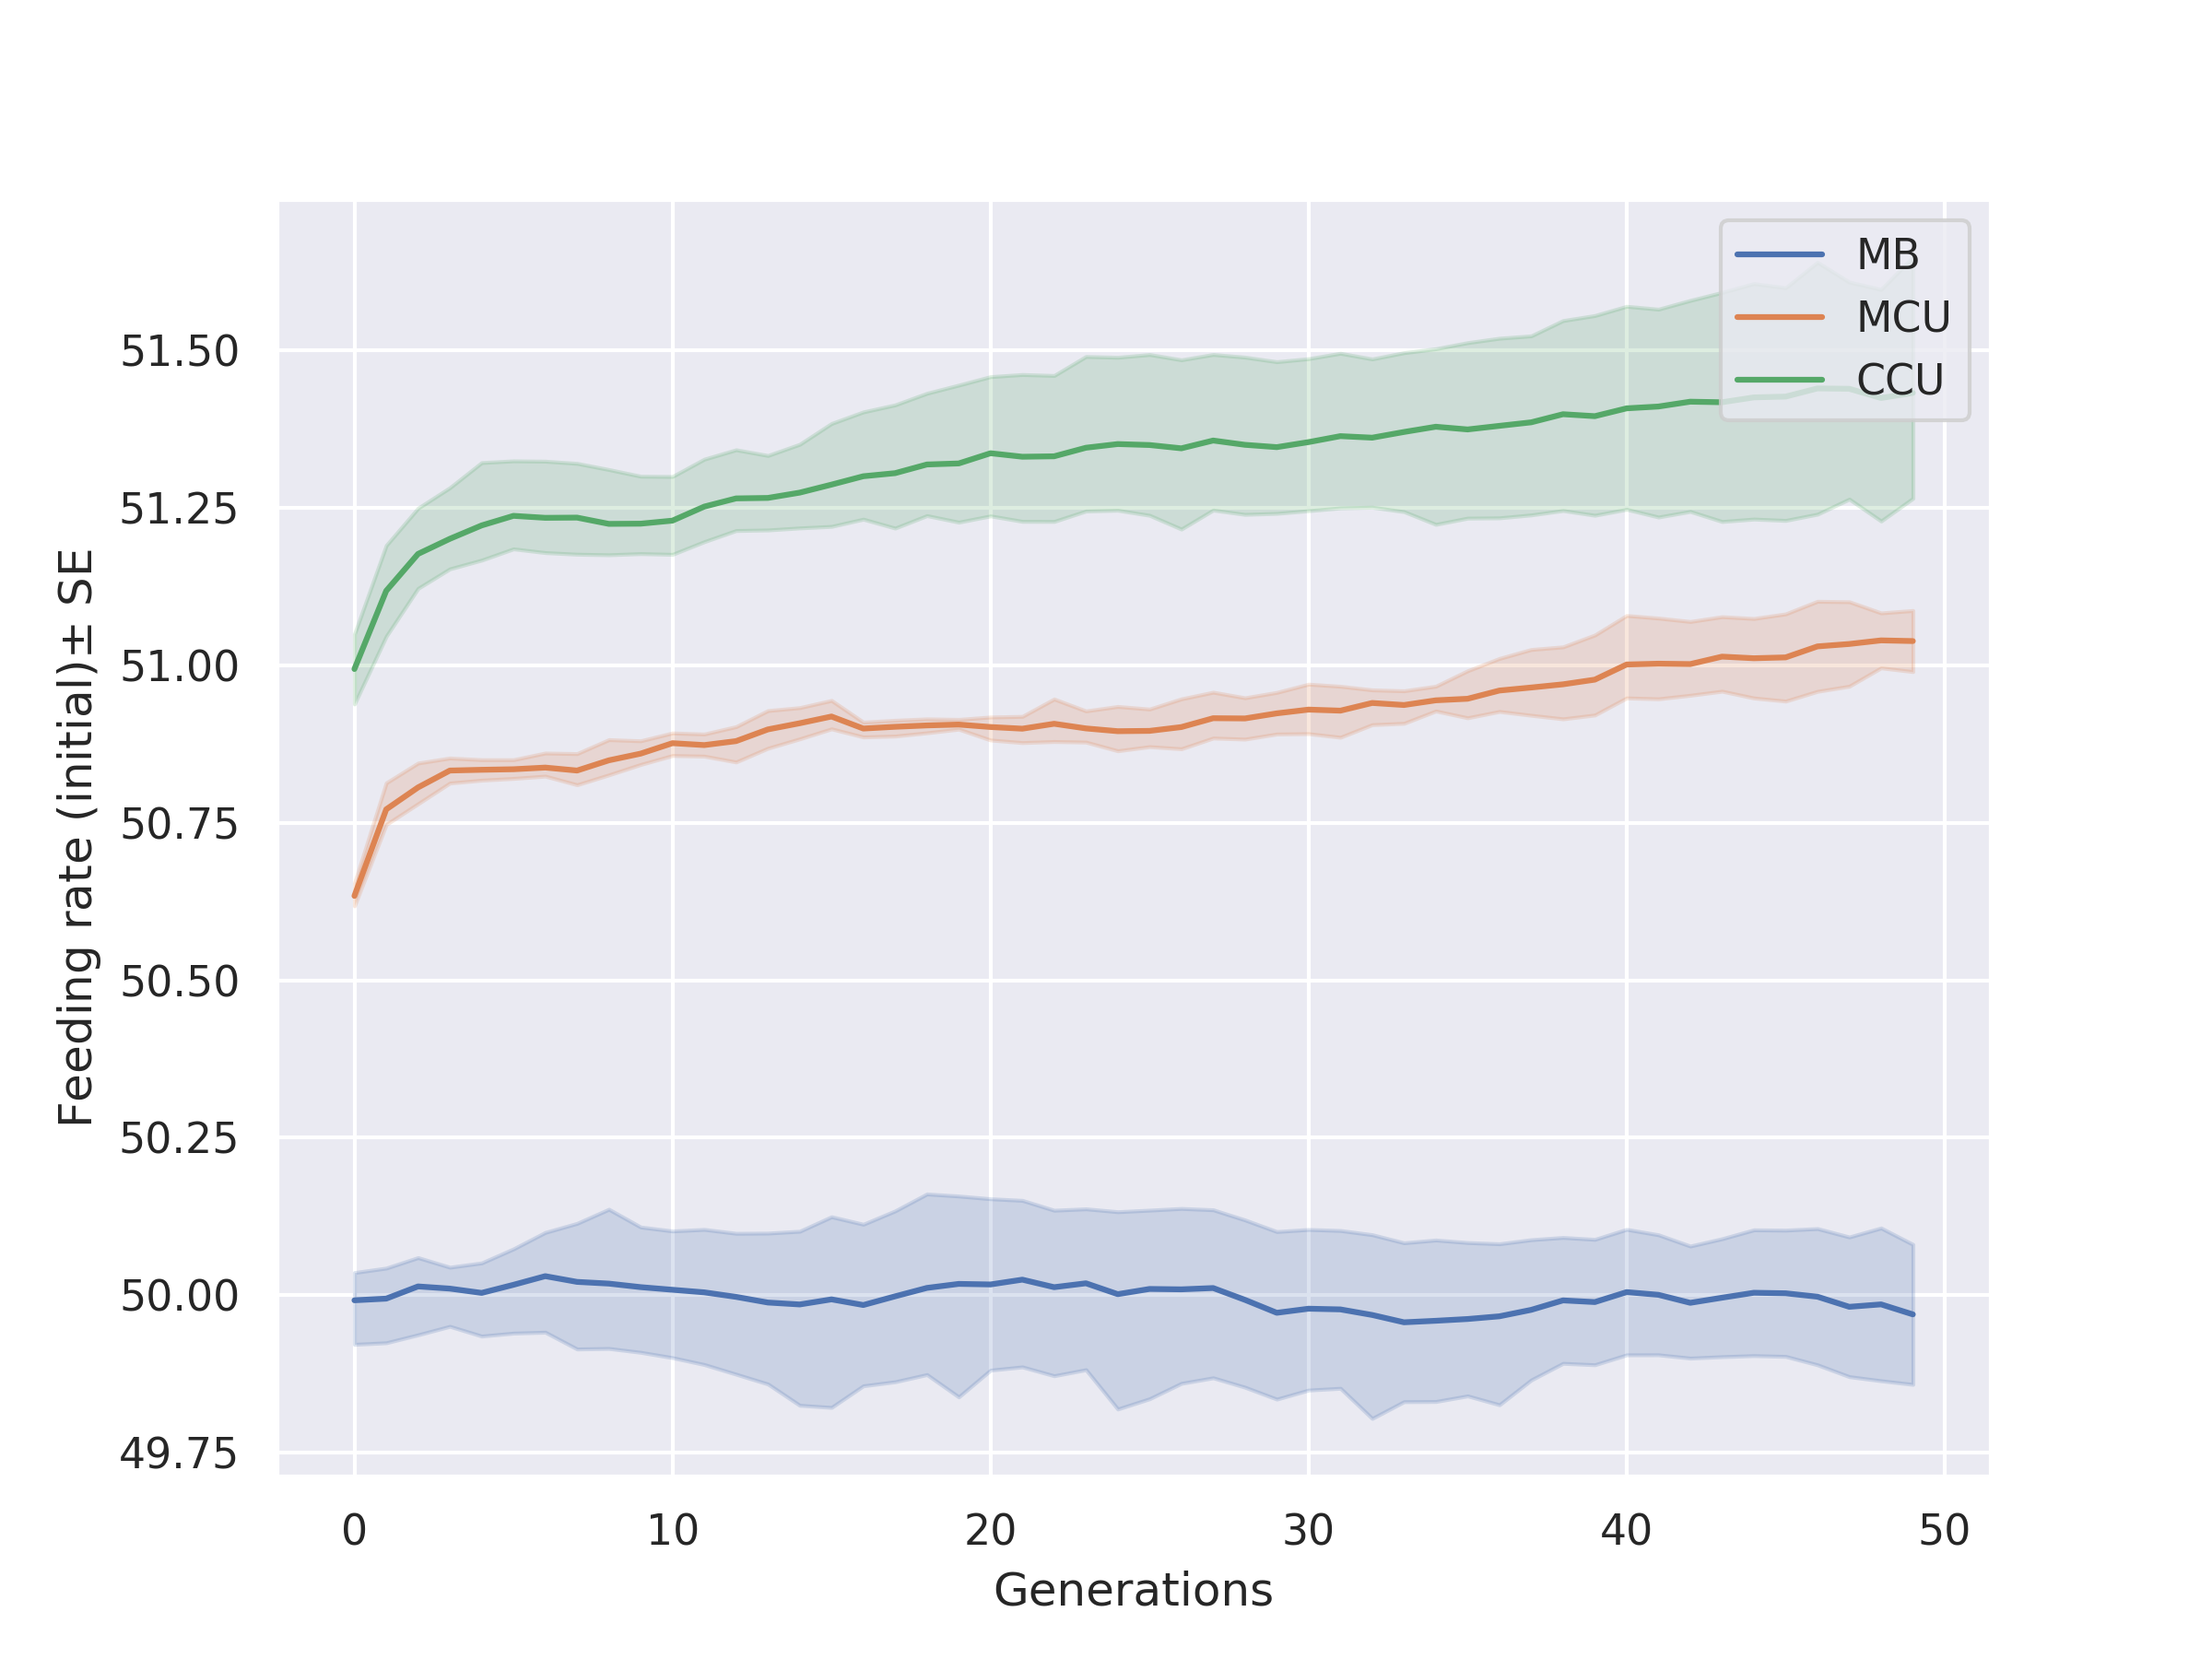
\includegraphics[trim = 0 0 50 50, clip, width=0.7\textwidth]{C4/Figs/fr}
  \caption{Timeseries for initial feeding rate}
  \label{fr}
\end{figure}
\begin{figure}[p]
  \centering
  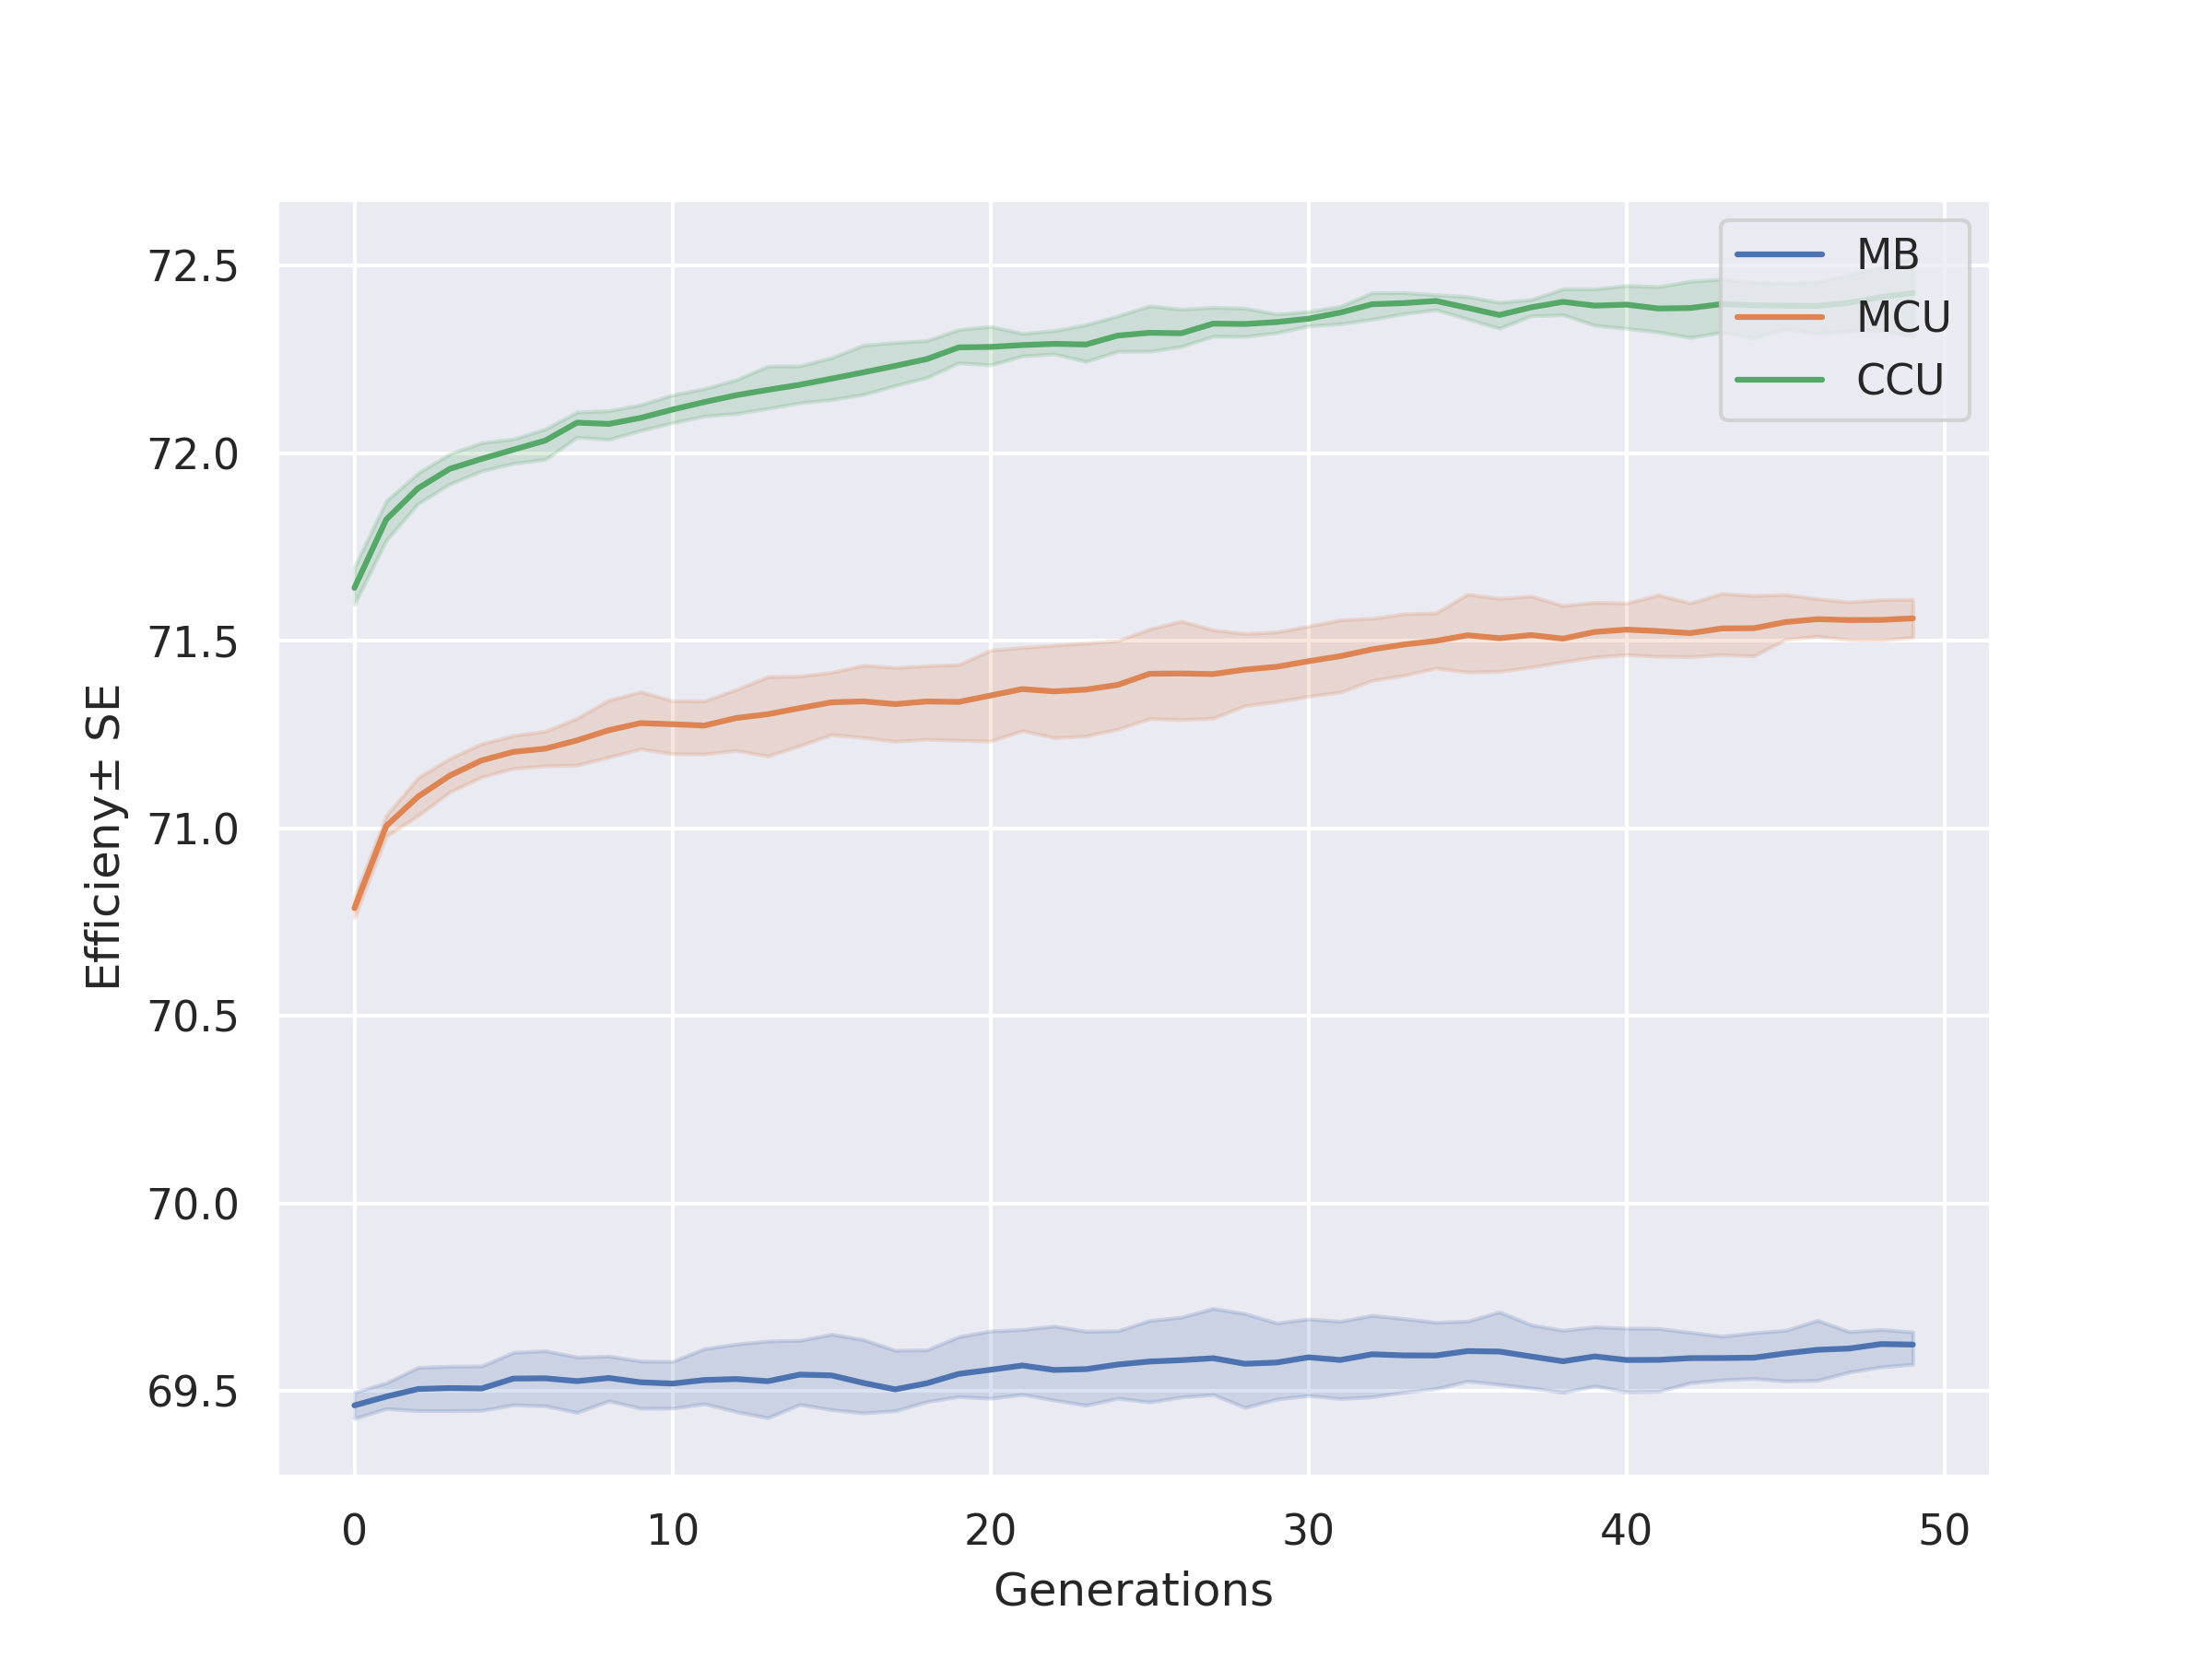
\includegraphics[trim = 0 0 50 50, clip, width=0.7\textwidth]{C4/Figs/eff}
  \caption{Timeseries for efficiency}
  \label{eff}
\end{figure}
\begin{figure}[p]
  \centering
  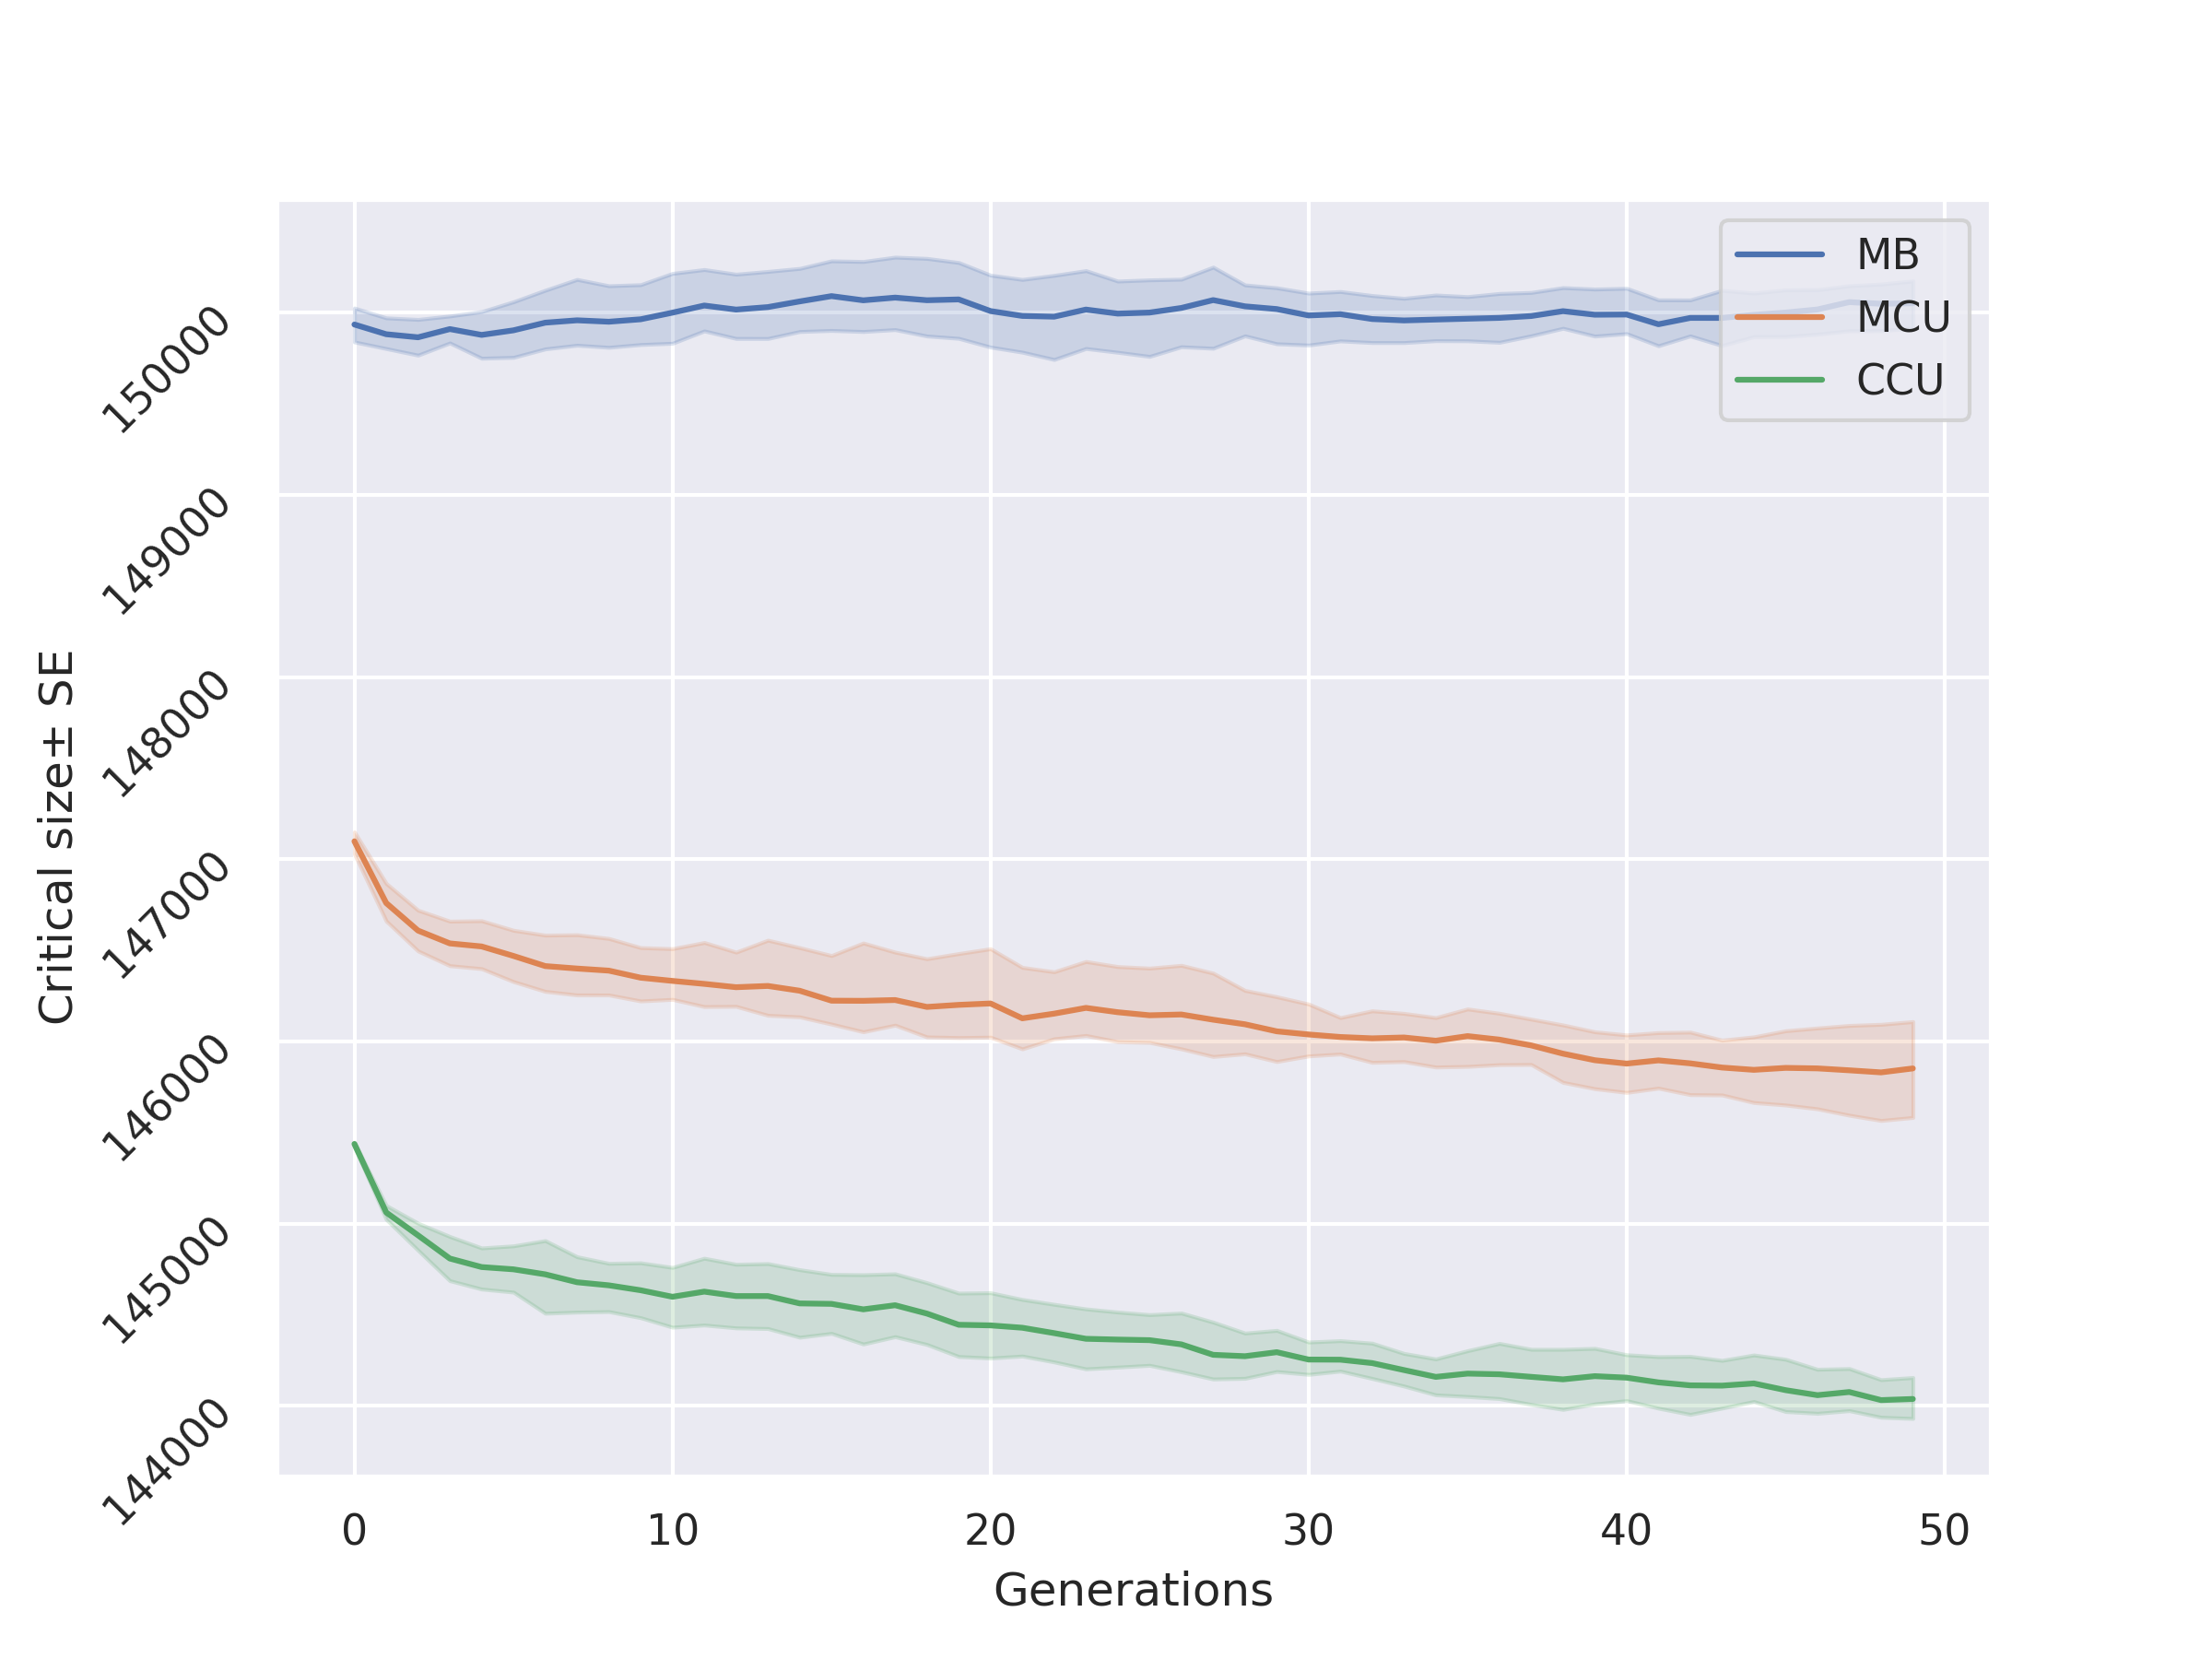
\includegraphics[trim = 0 0 50 50, clip, width=0.7\textwidth]{C4/Figs/mc}
  \caption{Timeseries for critical size}
  \label{mc}
\end{figure}

\newpage
\section{Effects of Variation on the Evolution of Larval Trait Parameters}
The stochasticity in the model comes from the initial variation in the larval trait parameters, given as certain variation in the respective initial distribution as well as from the heritability of the mid-parent value during the inheritance of the larval trait parameters. The simulations show how these sources of variations play an important role in determining the evolutionary routes taken to achieve greater competitive ability by having maximum survivorship.
\begin{figure}[t]
  \centering
  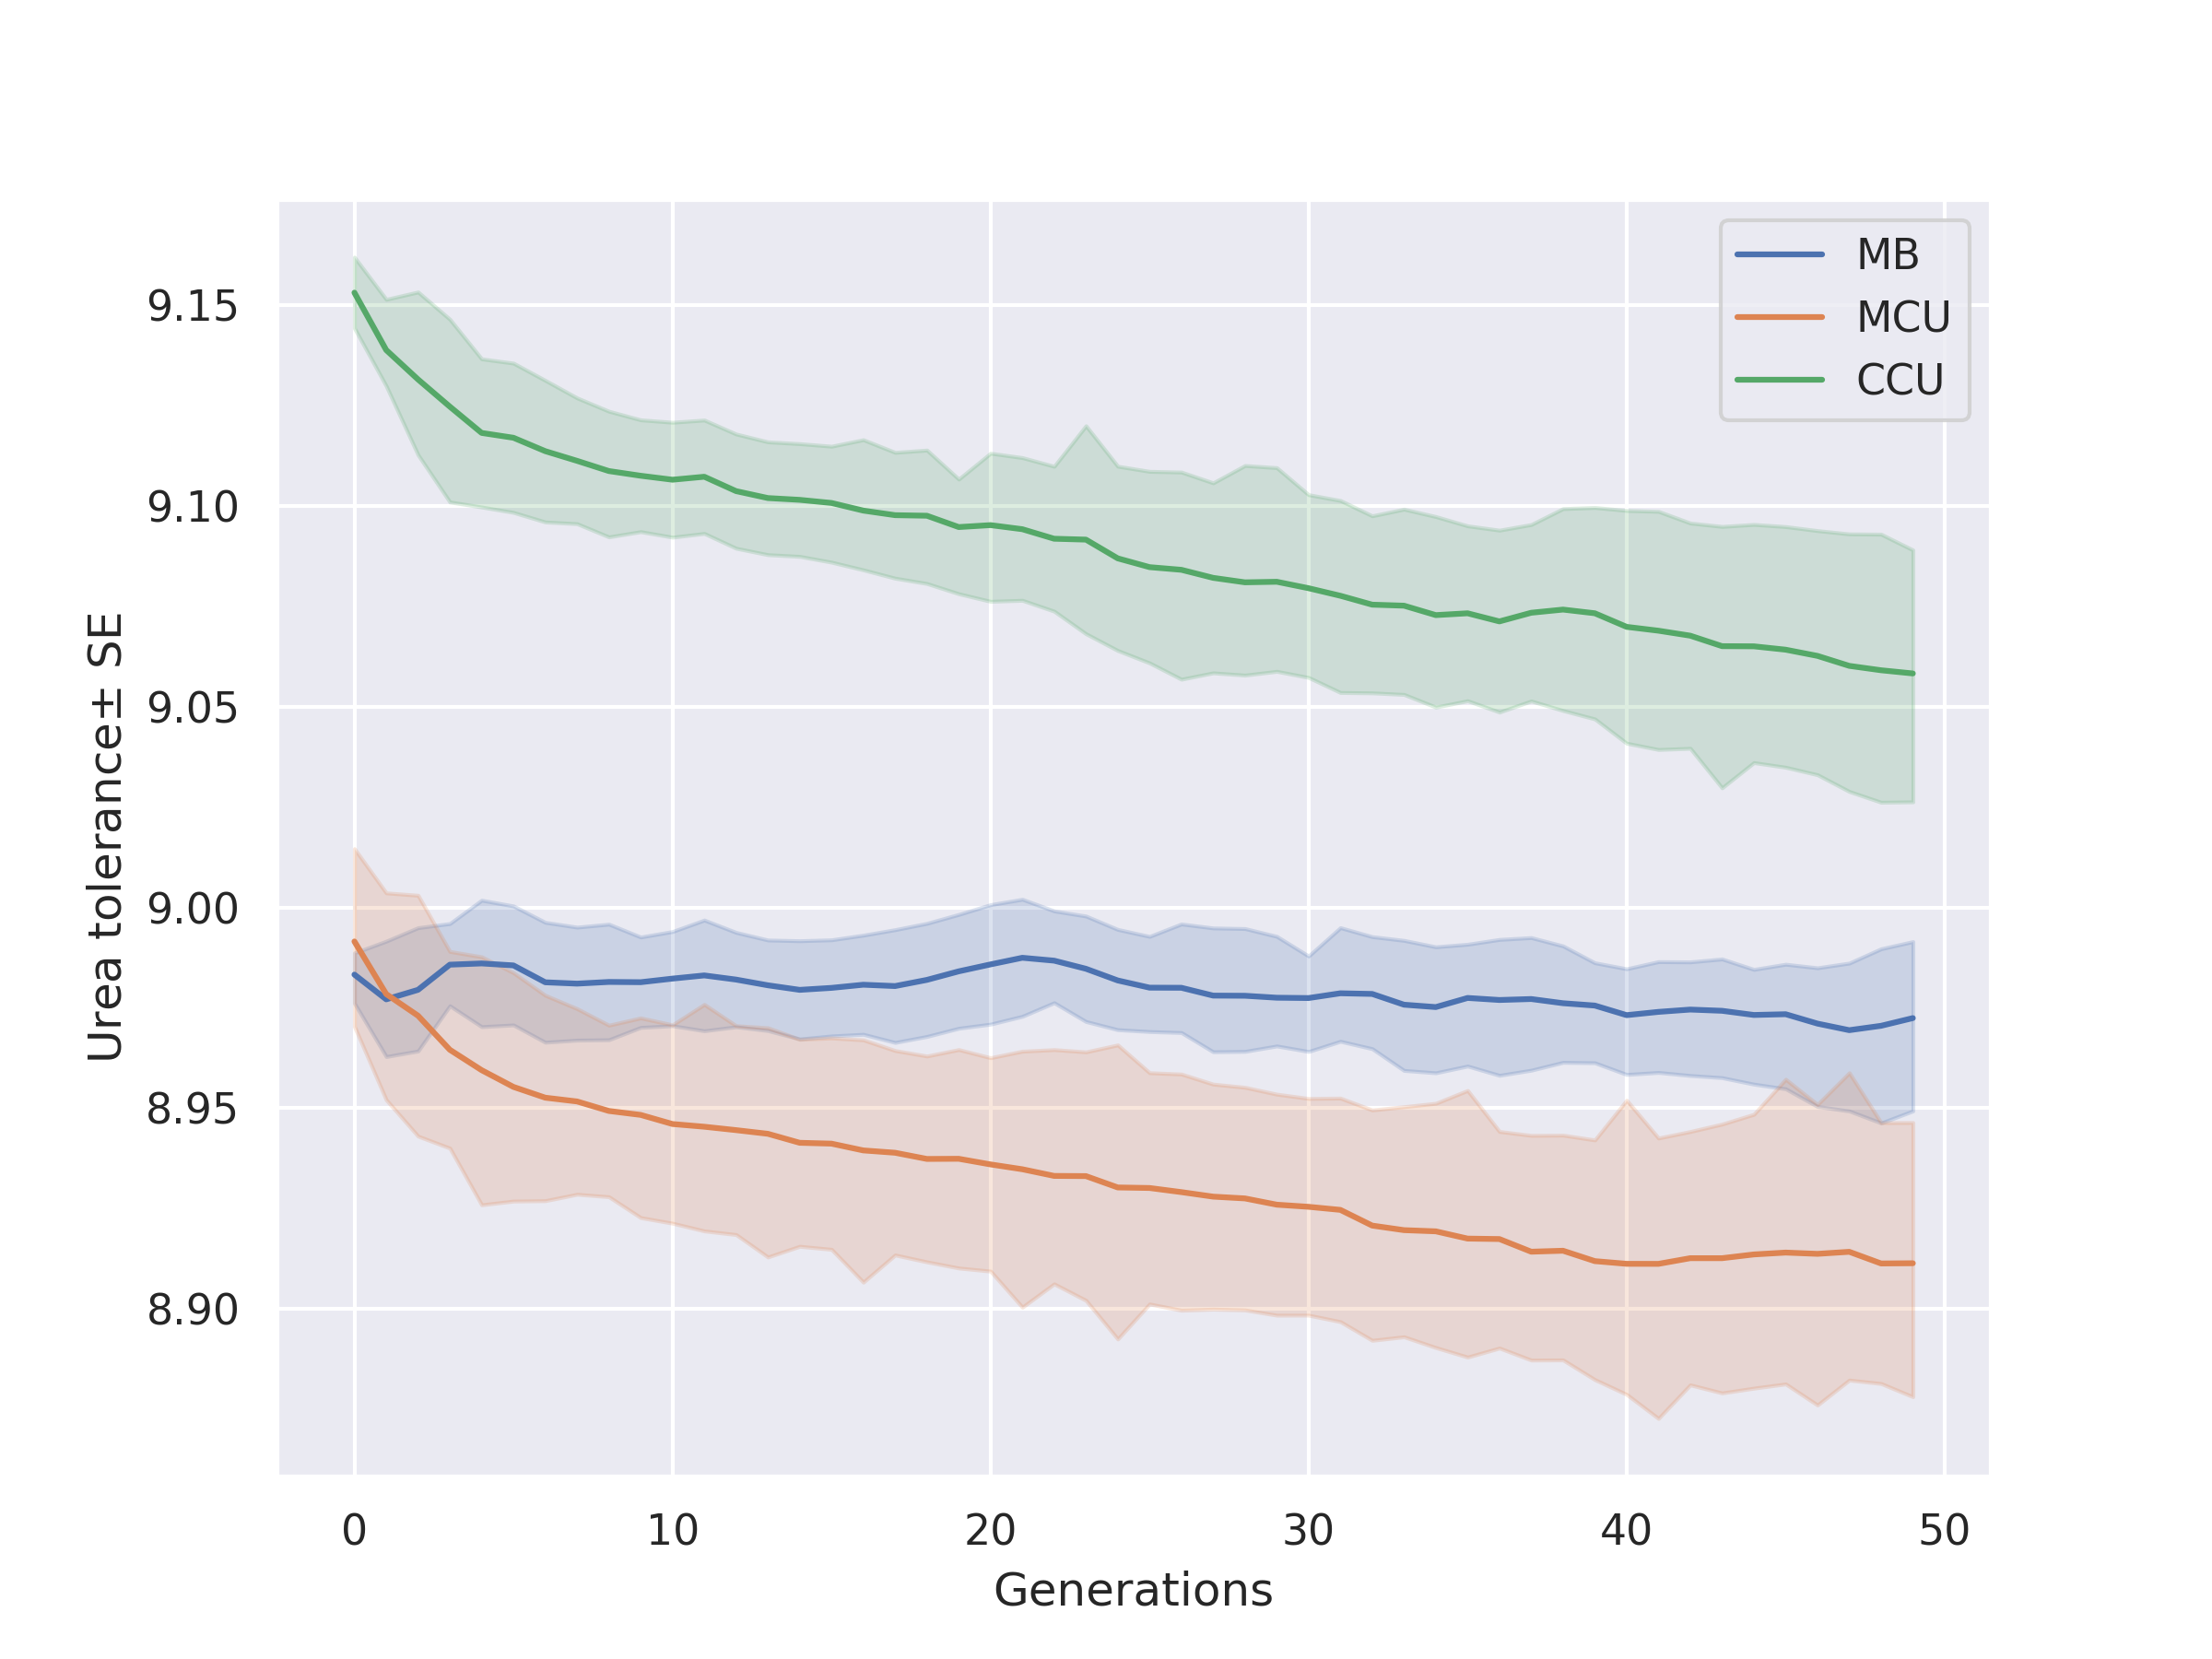
\includegraphics[trim = 0 0 50 50, clip, width=0.7\textwidth]{C4/Figs/wtol}
  \caption{Timeseries for waste tolerance}
  \label{wtol}
\end{figure}
\subsection{Variation in the Initial Distribution of Larval Trait Parameters}
In the initial distributions of all trait values, the variotion comes from the standard deviation given for each distribution. After $50^{th}$ generation, the initial variation in these trait distributions determine the maximum mean trait value that can be achieved to increase the fitness. From fig~\ref{fig:ivar_fr_eff} - fig~\ref{fig:ivar_mc_eff}, it is clear that differences in variation of these trait values, mean trait values reached are different for different combinations of intial variation in trait values.
\begin{figure}[p]
  \subfloat{
  \centering
  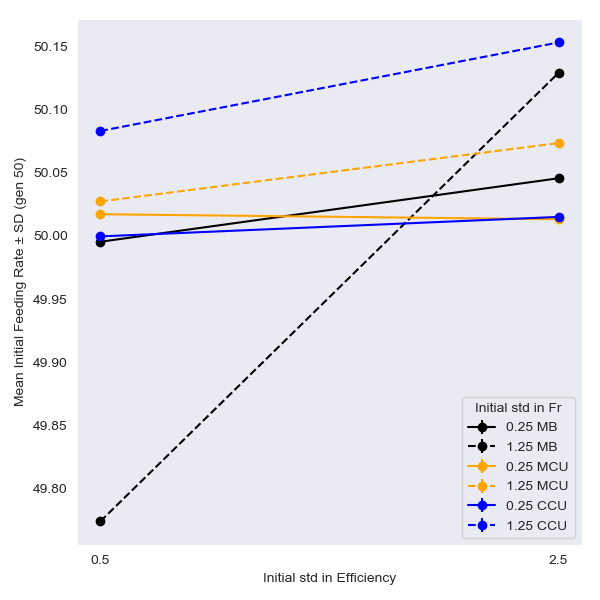
\includegraphics[width=0.5\textwidth]{C4/Figs/ivar/fr_eff_fr50}
  }
  \subfloat{
  \centering
  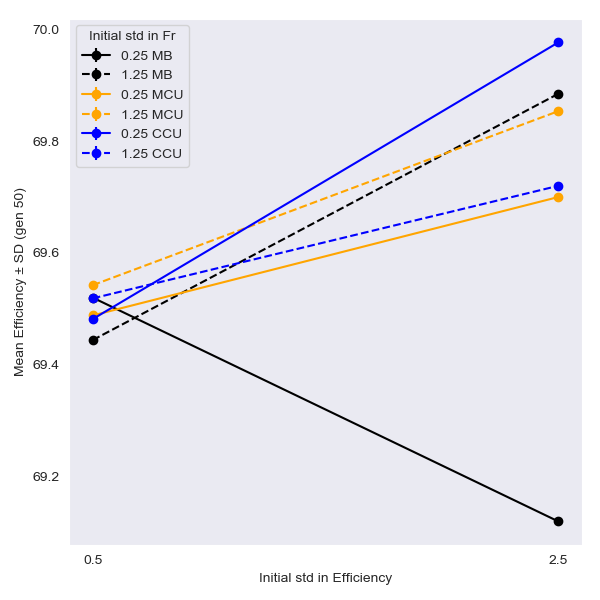
\includegraphics[width=0.5\textwidth]{C4/Figs/ivar/fr_eff_eff50}
  }\\
  \subfloat{
  \centering
  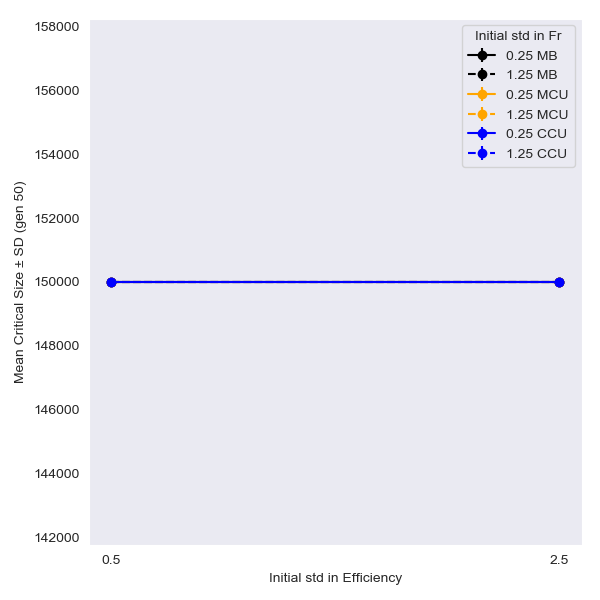
\includegraphics[width=0.5\textwidth]{C4/Figs/ivar/fr_eff_mc50}
  }
  \subfloat{
  \centering
  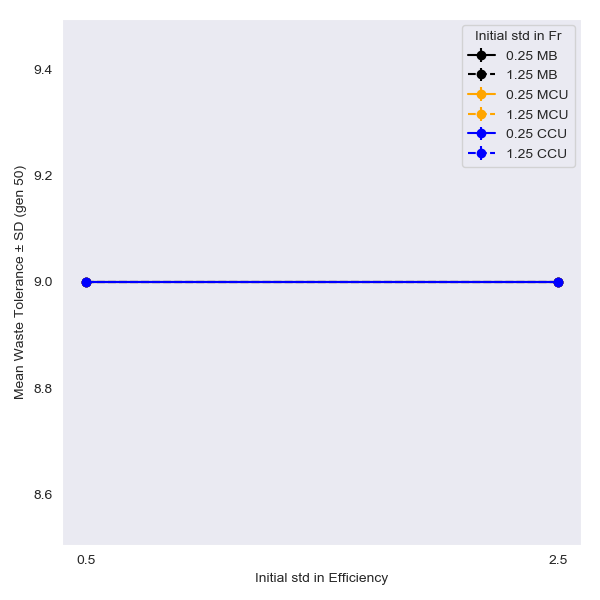
\includegraphics[width=0.5\textwidth]{C4/Figs/ivar/fr_eff_wtol50}
  }
  \caption{Effect of initial variation in initial feeding rate and efficiency on mean trait values at generation 50.}
  \label{fig:ivar_fr_eff}
\end{figure}
\begin{figure}[p]
  \subfloat{
  \centering
  \includegraphics[width=0.5\textwidth]{C4/Figs/ivar/fr_mc_fr50}
  }
  \subfloat{
  \centering
  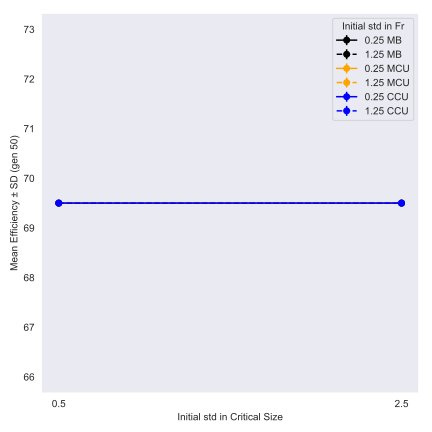
\includegraphics[width=0.5\textwidth]{C4/Figs/ivar/fr_mc_eff50}
  }\\
  \subfloat{
  \centering
  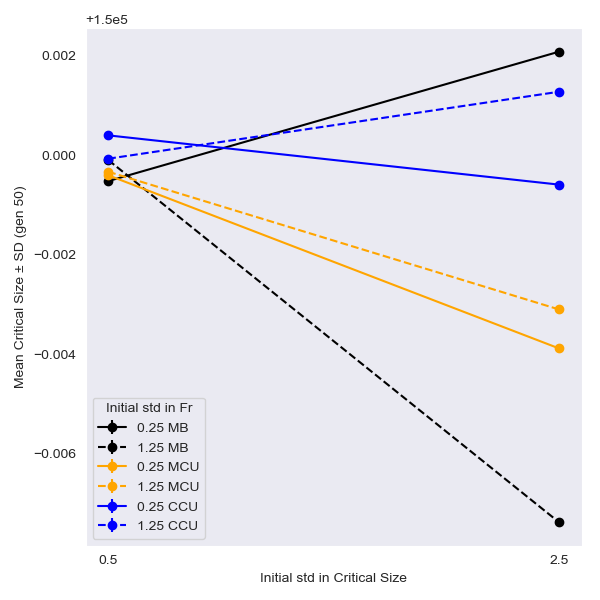
\includegraphics[width=0.5\textwidth]{C4/Figs/ivar/fr_mc_mc50}
  }
  \subfloat{
  \centering
  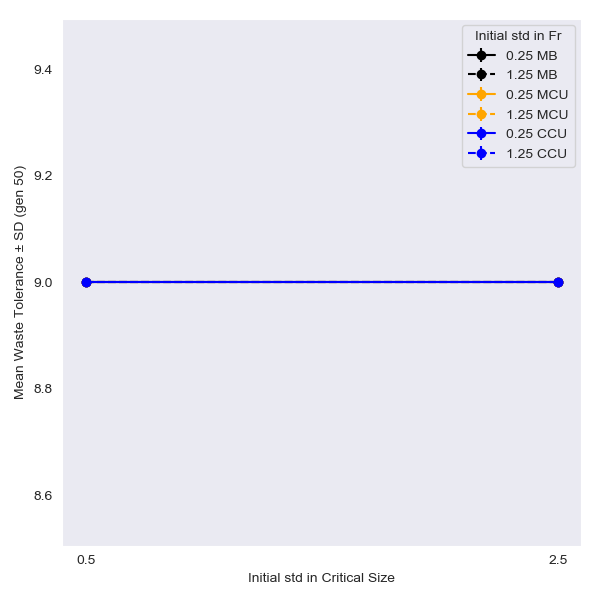
\includegraphics[width=0.5\textwidth]{C4/Figs/ivar/fr_mc_wtol50}
  }
  \caption{Effect of initial variation in initial feeding rate and critical size on mean trait values at generation 50.}
  \label{fig:ivar_fr_mc}
\end{figure}
\begin{figure}[p]
  \subfloat{
  \centering
  \includegraphics[width=0.5\textwidth]{C4/Figs/ivar/mc_eff_fr50}
  }
  \subfloat{
  \centering
  \includegraphics[width=0.5\textwidth]{C4/Figs/ivar/mc_eff_eff50}
  }\\
  \subfloat{
  \centering
  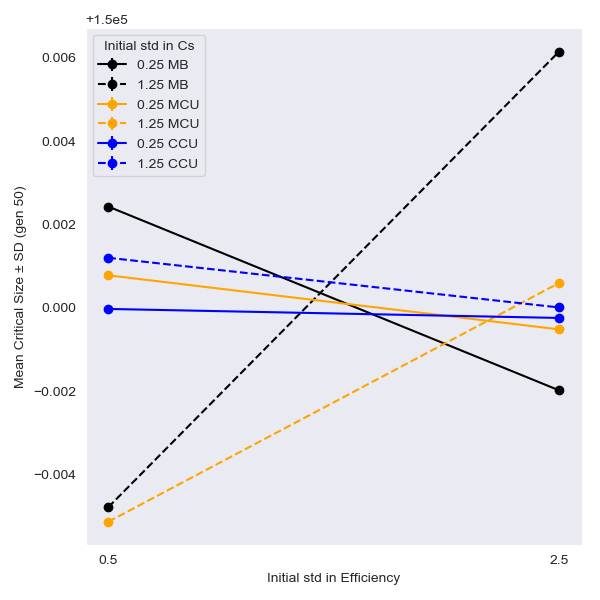
\includegraphics[width=0.5\textwidth]{C4/Figs/ivar/mc_eff_mc50}
  }
  \subfloat{
  \centering
  \includegraphics[width=0.5\textwidth]{C4/Figs/ivar/mc_eff_wtol50}
  }
  \caption{Effect of initial variation in critical size and efficiency on mean trait values at generation 50.}
  \label{fig:ivar_mc_eff}
\end{figure}

\newpage
\subsection{Heritability of Mid-parent Value}
\begin{figure}[h]
  \subfloat{
  \centering
  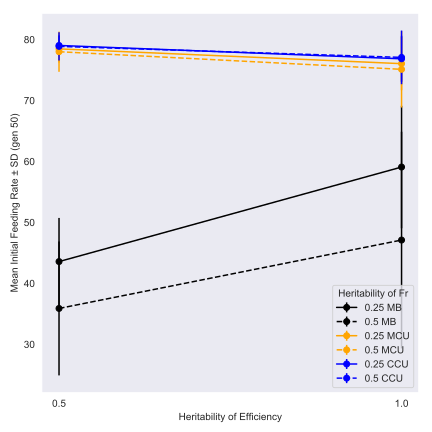
\includegraphics[width=0.5\textwidth]{C4/Figs/hrt/fr_eff_fr50}
  }
  \subfloat{
  \centering
  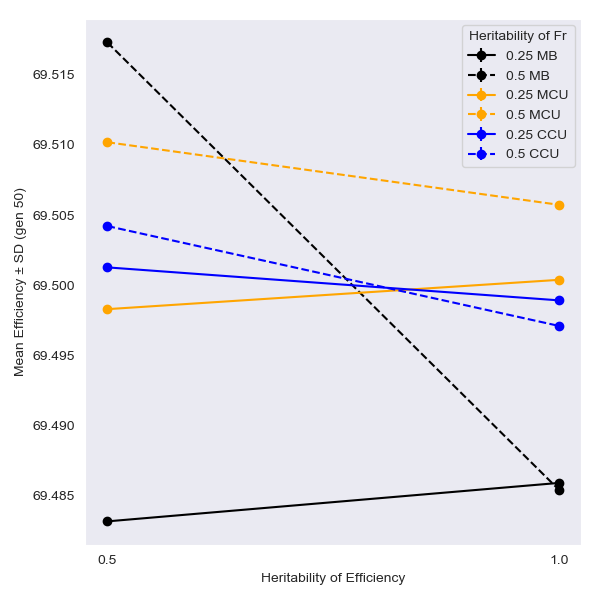
\includegraphics[width=0.5\textwidth]{C4/Figs/hrt/fr_eff_eff50}
  }\\
  \subfloat{
  \centering
  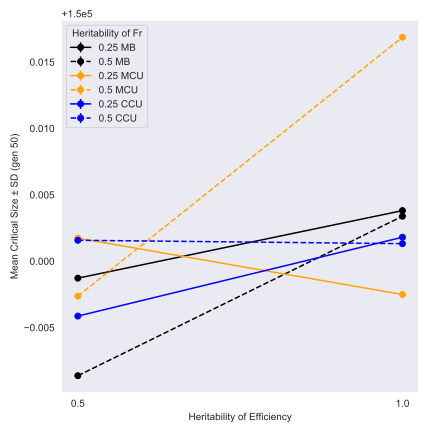
\includegraphics[width=0.5\textwidth]{C4/Figs/hrt/fr_eff_mc50}
  }
  \subfloat{
  \centering
  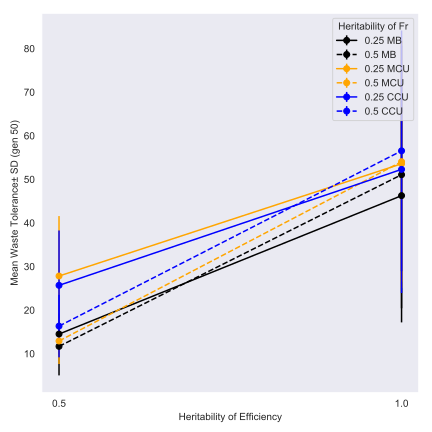
\includegraphics[width=0.5\textwidth]{C4/Figs/hrt/fr_eff_wtol50}
  }
  \caption{Effect of heritability in initial feeding rate and efficiency on mean trait values at generation 50.}
  \label{fig:hrt_fr_eff}
\end{figure}
\begin{figure}[p]
  \subfloat{
  \centering
  \includegraphics[width=0.5\textwidth]{C4/Figs/hrt/fr_mc_fr50}
  }
  \subfloat{
  \centering
  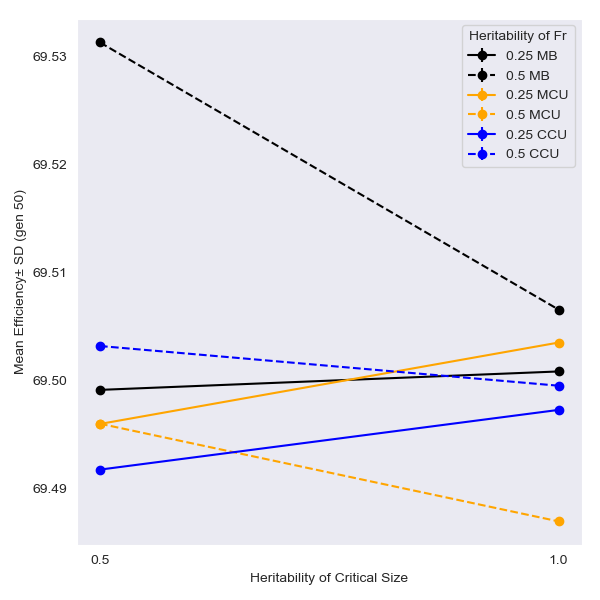
\includegraphics[width=0.5\textwidth]{C4/Figs/hrt/fr_mc_eff50}
  }\\
  \subfloat{
  \centering
  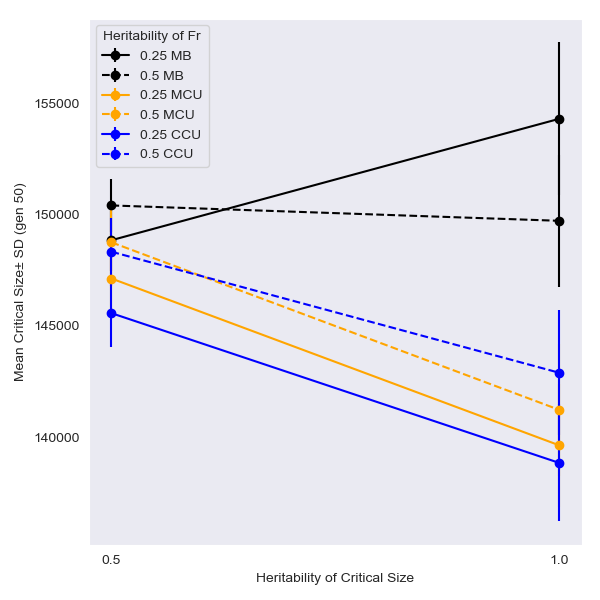
\includegraphics[width=0.5\textwidth]{C4/Figs/hrt/fr_mc_mc50}
  }
  \subfloat{
  \centering
  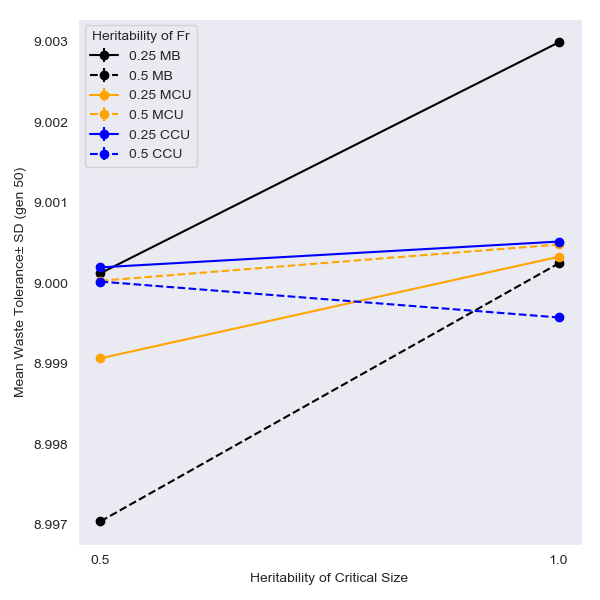
\includegraphics[width=0.5\textwidth]{C4/Figs/hrt/fr_mc_wtol50}
  }
  \caption{Effect of heritability in initial feeding rate and critical size on mean trait values at generation 50.}
  \label{fig:hrt_fr_mc}
\end{figure}
\begin{figure}[p]
  \subfloat{
  \centering
  \includegraphics[width=0.5\textwidth]{C4/Figs/hrt/mc_eff_fr50}
  }
  \subfloat{
  \centering
  \includegraphics[width=0.5\textwidth]{C4/Figs/hrt/mc_eff_eff50}
  }\\
  \subfloat{
  \centering
  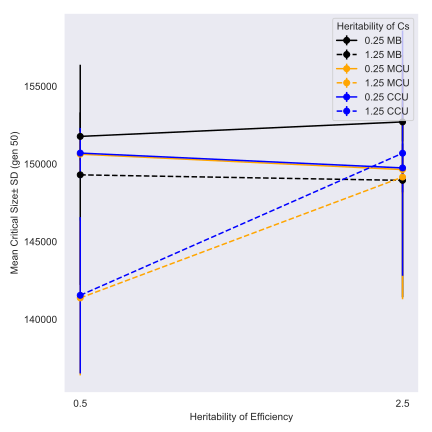
\includegraphics[width=0.5\textwidth]{C4/Figs/hrt/mc_eff_mc50}
  }
  \subfloat{
  \centering
  \includegraphics[width=0.5\textwidth]{C4/Figs/hrt/mc_eff_wtol50}
  }
  \caption{Effect of heritability in critical size and efficiency on mean trait values at generation 50.}
  \label{fig:hrt_mc_eff}
\end{figure}
\pagebreak
